% Soutenance 5MLDE : chaîne MLOps de prévision des ventes
% Compilation : latexmk -pdf presentation.tex   (ou pdflatex deux fois)
\documentclass[aspectratio=169,11pt]{beamer}

% ------------------------------------------------------------------ à compléter
\newcommand{\auteur}{Nema Elisée Kourouma \and Ju-heon Hwang \and Ahmed Chaudhry}
\newcommand{\etablissement}{SUPINFO}

\usetheme[progressbar=frametitle,numbering=fraction,sectionpage=none]{metropolis}
\usepackage[T1]{fontenc}
\usepackage[utf8]{inputenc}
\usepackage{lmodern}
\usepackage[french]{babel}
\usepackage{booktabs}
\usepackage{tabularx}
\usepackage{amsmath}
\usepackage{tikz}
\usetikzlibrary{positioning,arrows.meta,fit,backgrounds,shapes.geometric}
\usepackage{pgfplots}
\pgfplotsset{compat=1.18}

% ------------------------------------------------------------------ couleurs
\definecolor{bleu}{HTML}{1F4E79}
\definecolor{bleuclair}{HTML}{DCE6F1}
\definecolor{vert}{HTML}{2E7D32}
\definecolor{orange}{HTML}{E07B00}
\definecolor{rouge}{HTML}{C62828}
\definecolor{gris}{HTML}{5F6368}
\definecolor{fondcode}{HTML}{F5F7FA}
\setbeamercolor{frametitle}{bg=bleu,fg=white}
\setbeamercolor{progress bar}{fg=orange,bg=bleuclair}
\setbeamercolor{title separator}{fg=orange}
\setbeamercolor{alerted text}{fg=orange}
\setbeamercolor{block title}{bg=bleuclair,fg=bleu}
\setbeamercolor{block body}{bg=fondcode}
\setbeamertemplate{itemize item}{\color{orange}\raisebox{0.15ex}{$\blacktriangleright$}}
\setbeamertemplate{itemize subitem}{\color{gris}--}

\newcommand{\code}[1]{\texttt{\detokenize{#1}}}
\newcommand{\chiffre}[2]{\begin{minipage}[t]{\linewidth}\centering
  {\Huge\bfseries\color{bleu}#1}\\[2pt]{\small\color{gris}#2}\end{minipage}}
% Capture : image si présente, sinon cadre gris
\newcommand{\capt}[2][\linewidth]{\IfFileExists{../captures/#2}%
  {\includegraphics[width=#1,height=0.72\textheight,keepaspectratio]{../captures/#2}}%
  {\fbox{\parbox[c][3cm][c]{0.8\linewidth}{\centering\small capture manquante : #2}}}}

\title{Une chaîne MLOps de bout en bout}
\subtitle{Prévision des ventes hebdomadaires par produit -- UCI Online Retail}
\author{\auteur}
\institute{5MLDE -- \etablissement}
\date{Novembre 2026}

\begin{document}

% ================================================================== titre
\maketitle

% ================================================================== 1
\begin{frame}{Le problème posé}
\small
\begin{columns}[T]
\column{0.55\textwidth}
\textbf{Un besoin métier : le réassort}
\begin{itemize}
  \item Un e-commerce britannique doit commander avant de vendre
  \item Trop de stock immobilise, pas assez fait perdre des ventes
  \item On prévoit la \alert{quantité vendue la semaine suivante}, pour les
        \alert{50 produits} les plus vendus
\end{itemize}
\vspace{6pt}
\textbf{Ce qui est évalué}
\begin{itemize}
  \item Pas le score du modèle
  \item La \alert{chaîne} : opérationnelle, reproductible, maintenable
\end{itemize}
\column{0.42\textwidth}
\begin{block}{Fil conducteur}
Le modèle n'est qu'un passager.\\[4pt]
Ce qui compte, c'est la chaîne qui le \textbf{fabrique}, le \textbf{contrôle}, le
\textbf{met en service}, le \textbf{surveille} et permet de \textbf{revenir en arrière}.
\end{block}
\end{columns}
\end{frame}

% ================================================================== 2
\begin{frame}{Les données et leur rejeu}
\begin{columns}[T]
\column{0.5\textwidth}
\textbf{UCI Online Retail}
\begin{itemize}
  \item 541\,909 lignes de facture, 12/2010 -- 12/2011
  \item Licence \alert{CC BY 4.0}, DOI 10.24432/C5BW33
  \item Archive vérifiée par \alert{SHA256 figé} : une autre archive est refusée
  \item Données hors Git, téléchargées par \code{retail data}
\end{itemize}
\column{0.47\textwidth}
\textbf{Simuler l'arrivée des données}
\begin{itemize}
  \item Rejeu \alert{semaine ISO par semaine ISO} : 51 lots
  \item Semaine de Noël absente : trou \emph{enregistré}, pas masqué
  \item Le lot N+1 apporte les ventes réelles de la semaine prévue en N
        $\Rightarrow$ \alert{feedback automatique}
  \item Anti-fuite : top 50 figé sur les 8 premières semaines
\end{itemize}
\end{columns}
\end{frame}

% ================================================================== 3
\begin{frame}{Architecture}
\centering
\resizebox{!}{0.8\textheight}{%
\begin{tikzpicture}[
  font=\small,
  bloc/.style={draw=bleu,fill=bleuclair,rounded corners=3pt,minimum width=2.25cm,
               minimum height=0.95cm,align=center,line width=0.6pt},
  stock/.style={draw=gris,fill=fondcode,cylinder,shape border rotate=90,aspect=0.18,
               minimum width=2.2cm,minimum height=1.05cm,align=center},
  ext/.style={draw=orange,fill=orange!10,rounded corners=3pt,minimum width=2.1cm,
               minimum height=0.9cm,align=center},
  fl/.style={-{Stealth[length=2.4mm]},line width=0.7pt,color=bleu},
  fb/.style={-{Stealth[length=2.2mm]},line width=0.6pt,color=vert,dashed},
  node distance=0.55cm and 0.5cm]
  \node[stock] (uci) {Archive UCI\\\scriptsize SHA256 figé};
  \node[bloc,right=of uci] (lots) {Lots ISO\\\scriptsize 51 semaines};
  \node[bloc,right=of lots] (qual) {Qualité\\\scriptsize Pandera};
  \node[bloc,right=of qual] (feat) {Features\\\scriptsize lags, moyenne};
  \node[bloc,right=of feat] (train) {Entraînement\\\scriptsize Ridge vs naïf};
  \node[stock,below=1.3cm of train] (mlf) {MLflow\\\scriptsize registre :5001};
  \node[bloc,left=1.1cm of mlf] (champ) {Champion\\\scriptsize export disque};
  \node[bloc,left=1.1cm of champ] (api) {API FastAPI\\\scriptsize :8001};
  \node[stock,left=1.1cm of api] (pg) {PostgreSQL\\\scriptsize :5437};
  \node[ext,below=1.25cm of api] (prom) {Prometheus\\\scriptsize :9091};
  \node[ext,left=of prom] (graf) {Grafana\\\scriptsize :3001};
  \node[ext,right=of prom] (loc) {Locust\\\scriptsize charge};
  \begin{scope}[on background layer]
    \node[draw=bleu!60,dashed,rounded corners=5pt,fit=(lots)(train),inner sep=7pt,
          label={[font=\scriptsize\bfseries,text=bleu,anchor=south east]north east:Prefect : un lot par tick}] {};
  \end{scope}
  \draw[fl] (uci) -- (lots);
  \draw[fl] (lots) -- (qual);
  \draw[fl] (qual) -- node[above,font=\scriptsize]{OK} (feat);
  \draw[fl] (feat) -- (train);
  \draw[fl] (train) -- node[right,font=\scriptsize]{enregistre} (mlf);
  \draw[fl] (mlf) -- node[above,font=\scriptsize]{promeut} (champ);
  \draw[fl] (champ) -- node[above,font=\scriptsize]{sert} (api);
  \draw[fl] (api) -- node[above,font=\scriptsize]{traces} (pg);
  \draw[fb] (qual.south) |- ++(0,-0.55) -| node[pos=0.25,above,font=\scriptsize,text=vert]{feedback auto} (pg.north);
  \draw[fl,color=rouge] (qual.north) -- ++(0,0.85) node[above,font=\scriptsize,text=rouge]{KO : arrêt + alerte};
  \draw[fl,color=orange] (prom) -- node[left,font=\scriptsize]{/metrics} (api);
  \draw[fl,color=orange] (graf) -- (prom);
  \draw[fl,color=orange] (graf.north) -- (pg.south);
  \draw[fl,color=orange] (loc) -- (api.south east);
\end{tikzpicture}}
\end{frame}

% ================================================================== 4
\begin{frame}{Choix techniques}
\small
\begin{tabularx}{\linewidth}{>{\bfseries}l l X}
\toprule
Besoin & Outil & Pourquoi\\
\midrule
Configuration & YAML + \code{.env} & règles relues en revue de code, secrets hors Git\\
Qualité & Pandera & schémas déclaratifs, contrôles bloquants, rapport par lot\\
Modèle & Ridge (scikit-learn) & simple, rapide, comparé à une prévision naïve\\
Registre & MLflow & runs, versions, alias \code{champion}/\code{challenger}, tags\\
Orchestration & Prefect & relances ciblées, historique, planification\\
Service & FastAPI & validation Pydantic, documentation automatique\\
Traces & PostgreSQL & partagé par l'API, le pipeline et Grafana\\
Supervision & Prometheus + Grafana & métriques, alertes, tableau de bord versionné\\
Charge & Locust + Docker & même protocole sur plusieurs limites CPU/mémoire\\
\bottomrule
\end{tabularx}
\vfill
\centering\footnotesize\color{gris}Tout tourne en local, sans service payant. Code : 131 tests, lint \code{ruff}, CI sur Python 3.11 à 3.13.
\end{frame}

% ================================================================== 5
\begin{frame}{Qualité des données : un contrôle qui bloque}
\begin{columns}[T]
\column{0.52\textwidth}
\textbf{Trois étapes, dans l'ordre}
\begin{enumerate}
  \item Schéma des factures : types, dates dans la semaine, volume, prix nuls
  \item Nettoyage \alert{tracé} : chaque ligne écartée est comptée et justifiée
  \item Schéma du panel produit $\times$ semaine
\end{enumerate}
\vspace{4pt}
Un échec $\Rightarrow$ pas de panel, \alert{pas d'entraînement}, alerte, curseur bloqué
\column{0.45\textwidth}
\begin{block}{Erreur de données $\neq$ panne}
\begin{itemize}
  \item Panne technique : Prefect \alert{relance} (2 fois, 10 s)
  \item Données invalides : \alert{jamais} relancées -- relancer un lot faux ne le rend pas juste
\end{itemize}
\end{block}
\vspace{4pt}
\small Démo : lot \code{2099-W01} rejeté par 3 contrôles, aucun entraînement.
\end{columns}
\end{frame}

% ================================================================== 6
\begin{frame}{Mise en service et retour arrière}
\small
\begin{columns}[T]
\column{0.5\textwidth}
\textbf{Une règle explicite}
\begin{enumerate}
  \item \alert{Enregistrer} seulement si le modèle bat la prévision naïve
  \item \alert{Promouvoir} si MAE $\leq$ champion, \emph{sur le même jeu de test}
\end{enumerate}
\vspace{4pt}
\textbf{Tout est tracé dans MLflow}
\begin{itemize}
  \item semaines utilisées, empreinte des variables
  \item paramètres, métriques, modèle signé
  \item décision écrite en tag
\end{itemize}
\vspace{4pt}
\textbf{Retour arrière} : \code{retail rollback} remet \code{previous_champion}
\column{0.48\textwidth}
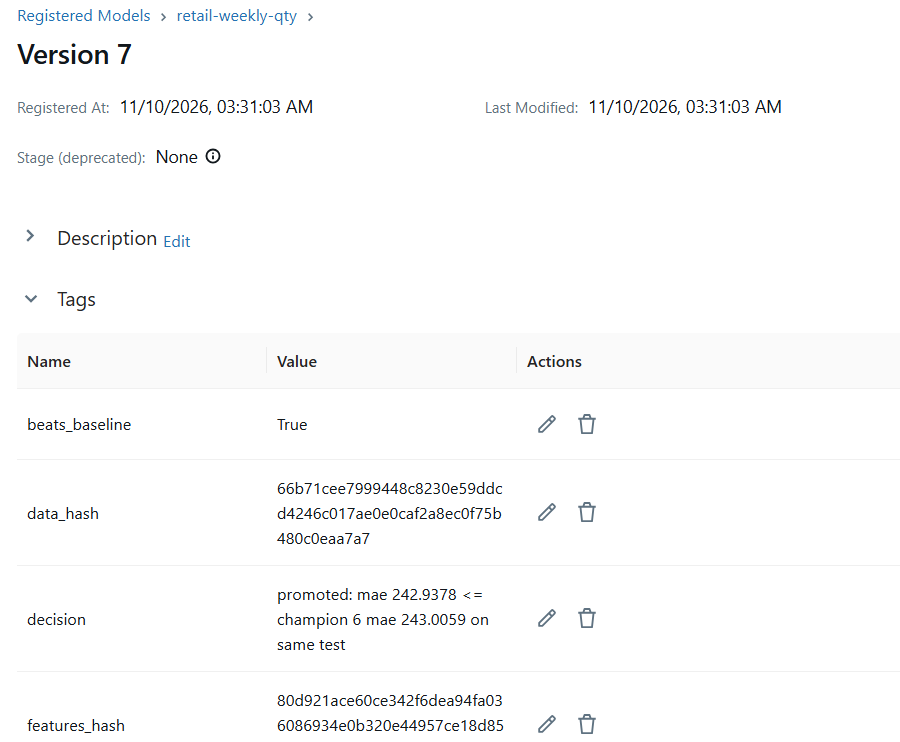
\includegraphics[width=\linewidth,height=0.78\textheight,keepaspectratio]{img/mlflow_v7.png}
\end{columns}
\end{frame}

% ================================================================== 7
\begin{frame}{Le registre : 7 versions promues automatiquement}
\centering
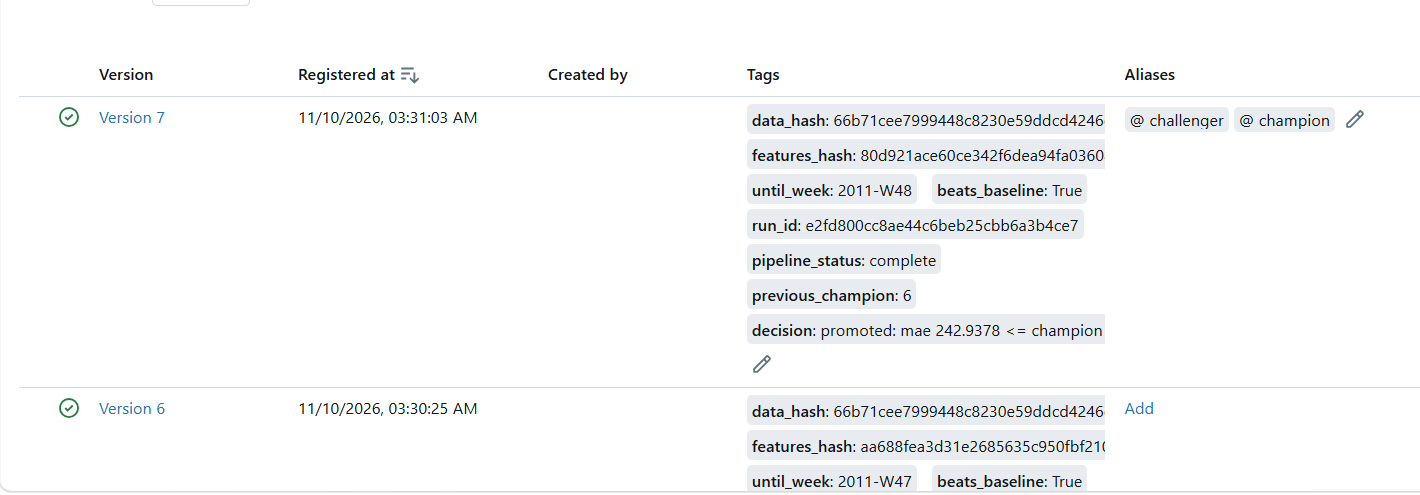
\includegraphics[width=0.98\linewidth]{img/mlflow_liste.png}

\vspace{4pt}
\small Chaque version porte la semaine d'entraînement, l'empreinte des variables, le champion précédent et la décision ; l'alias \code{champion} désigne la version servie.
\end{frame}

% ================================================================== 8
\begin{frame}{Orchestration avec Prefect}
\begin{columns}[T]
\column{0.34\textwidth}
\small
\textbf{Un lot par exécution}
\begin{enumerate}
  \item choisir la semaine suivante
  \item valider le lot
  \item feedback automatique
  \item entraîner, enregistrer, promouvoir
  \item prévoir N+1 via l'API
\end{enumerate}
\vspace{4pt}
\small Déclenché toutes les 10 min, une exécution à la fois, verrou anti-concurrence.
\column{0.64\textwidth}
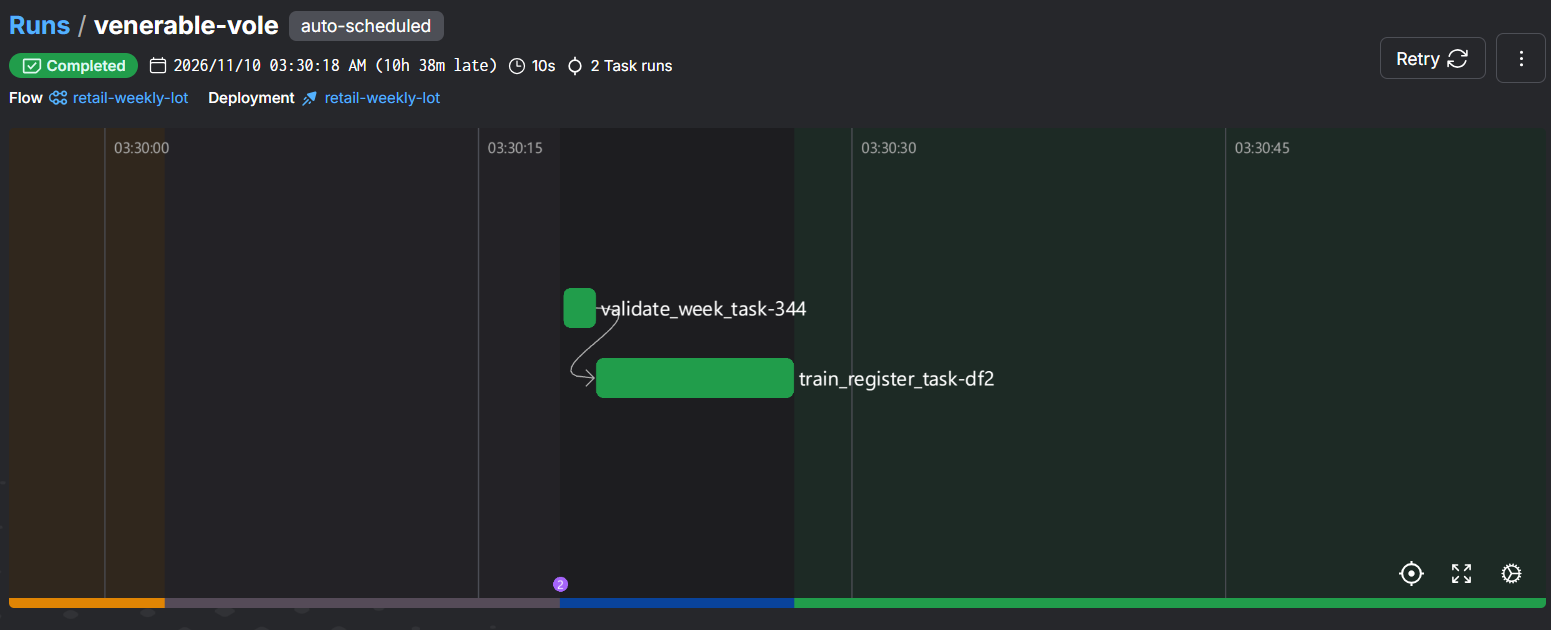
\includegraphics[width=\linewidth]{img/prefect.png}\\[3pt]
\footnotesize Exécution planifiée : validation de W47, puis entraînement et enregistrement de la v6 en 10 s.
\end{columns}
\end{frame}

% ================================================================== 9
\begin{frame}{API de prédiction}
\begin{columns}[T]
\column{0.5\textwidth}
\footnotesize
\begin{tabular}{ll}
\toprule
Route & Rôle\\
\midrule
\code{POST /predict} & un produit, une semaine\\
\code{POST /predict/batch} & les 50 produits\\
\code{POST /feedback} & quantité réelle\\
\code{GET /health} & version, base, mode dégradé\\
\code{GET /model} & version, WAPE de production\\
\code{GET /metrics} & Prometheus\\
\bottomrule
\end{tabular}
\column{0.48\textwidth}
\small
\begin{itemize}
  \item Entrées validées : 404 produit inconnu, 422 semaine invalide ou hors horizon
  \item \alert{Version renvoyée} dans chaque réponse (\code{X-Model-Version})
  \item \code{prediction_id} pour rattacher le retour terrain
  \item Rechargement atomique du champion
  \item MLflow injoignable $\Rightarrow$ \alert{mode dégradé} sur le champion local
\end{itemize}
\end{columns}
\end{frame}

% ================================================================== 10
\begin{frame}{Persistance et retours terrain}
\begin{columns}[T]
\column{0.5\textwidth}
\textbf{Tout est conservé dans PostgreSQL}
\begin{itemize}
  \item prédictions : version, durée, statut, erreur
  \item feedbacks : réel, prédit, erreur
  \item exécutions du pipeline, alertes
\end{itemize}
\vspace{4pt}
\textbf{Le service avant la trace}
\begin{itemize}
  \item écriture en file, par lots
  \item base coupée : l'API répond toujours, les pertes sont \alert{comptées}
\end{itemize}
\column{0.47\textwidth}
\begin{block}{Boucle fermée}
Le lot de la semaine N+1 ferme les prédictions faites pour N+1 :\\[3pt]
$\Rightarrow$ \alert{WAPE de production par version}, en plus de la MAE d'entraînement.
\end{block}
\vspace{4pt}
\small Trafic de test marqué \code{X-Load-Test}, exclu des retours et de la WAPE.
\end{columns}
\end{frame}

% ================================================================== 11
\begin{frame}{Supervision : la coupure de PostgreSQL vue par Grafana}
\centering
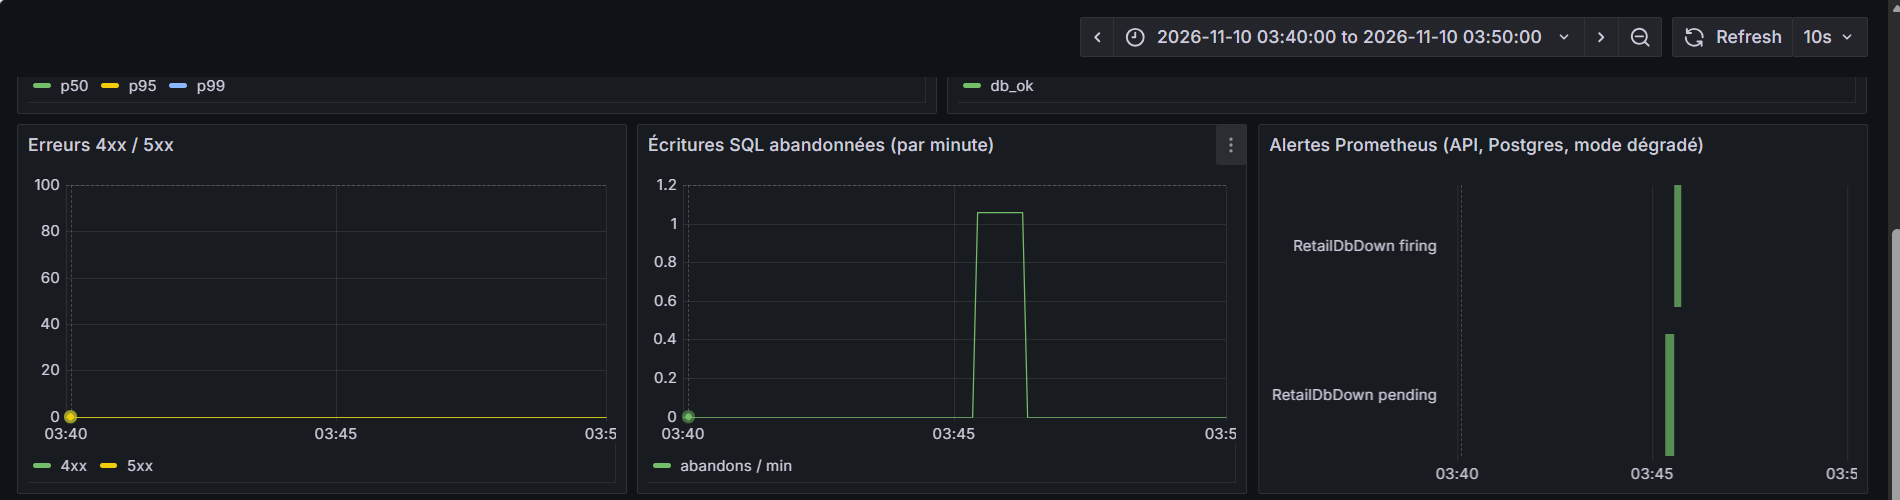
\includegraphics[width=\linewidth]{img/grafana_incident.png}

\vspace{6pt}
\small
\begin{columns}[T]
\column{0.48\textwidth}
\begin{itemize}
  \item Coupure volontaire de la base vers 03\,h\,45
  \item Les écritures perdues sont \alert{comptées}, pas silencieuses
\end{itemize}
\column{0.48\textwidth}
\begin{itemize}
  \item \code{RetailDbDown} : en attente, puis \alert{déclenchée}
  \item Aucune erreur 5xx : l'API a continué de répondre
\end{itemize}
\end{columns}
\end{frame}

\begin{frame}{Supervision : suivi du modèle et du pipeline}
\begin{columns}[c]
\column{0.68\textwidth}
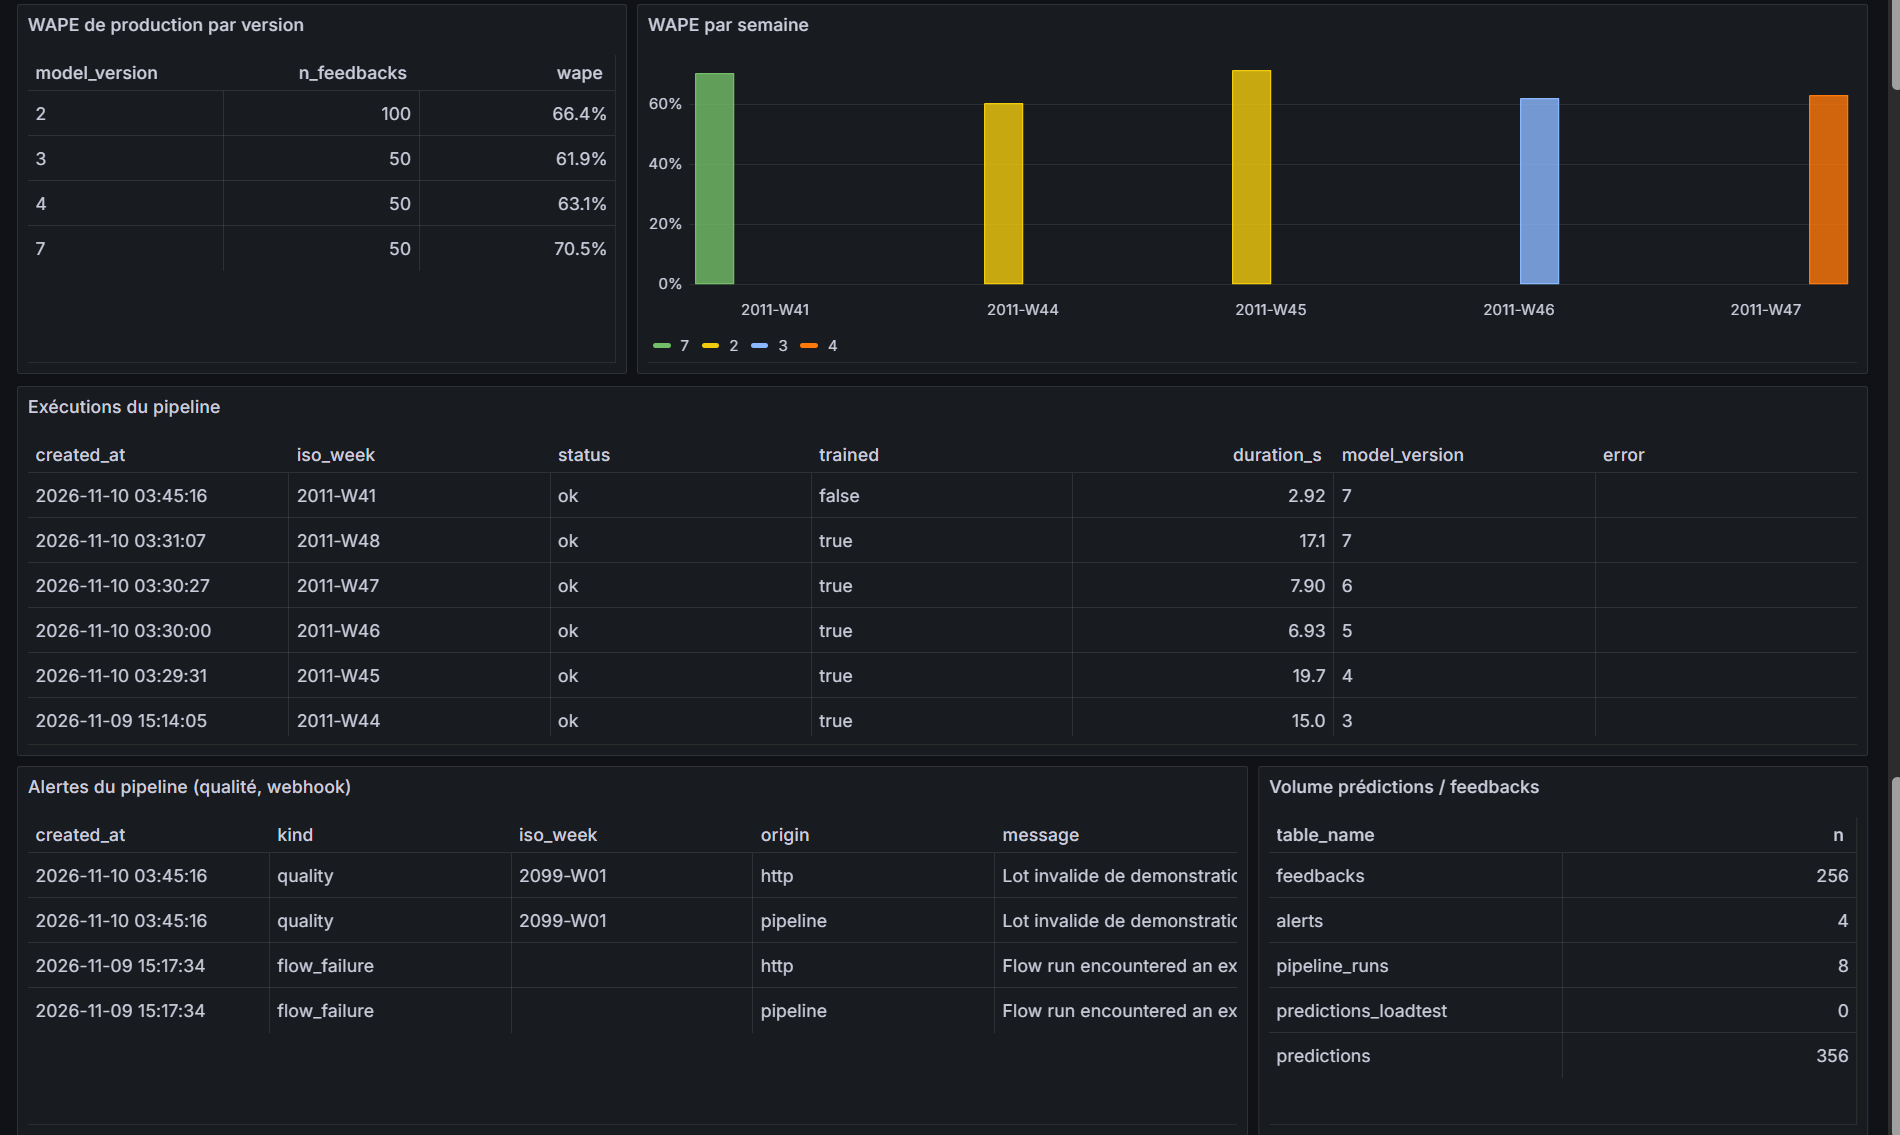
\includegraphics[width=\linewidth,height=0.8\textheight,keepaspectratio]{img/grafana_suivi.png}
\column{0.3\textwidth}
\small
\begin{itemize}
  \item WAPE de production par version et par semaine
  \item Exécutions : semaine, durée, version
  \item Alertes du pipeline
  \item Volumes de traces
\end{itemize}
\vspace{4pt}
\footnotesize 4 alertes Prometheus : API arrêtée, base injoignable, mode dégradé, taux de 5xx.
\end{columns}
\end{frame}

% ================================================================== 12
\begin{frame}{Tests de charge : le protocole}
\begin{columns}[T]
\column{0.5\textwidth}
\begin{itemize}
  \item Locust : 70\,\% \code{/predict}, 20\,\% lot, 10\,\% santé
  \item Paliers de 2 à 320 utilisateurs, 45 s chacun
  \item 3 conteneurs limités : 1, 2 et 4 workers
  \item \alert{Capacité} = dernier palier avec p95 $<$ 200 ms et 0 erreur
\end{itemize}
\column{0.47\textwidth}
\begin{block}{La première série a servi}
Elle a révélé deux défauts :
\begin{itemize}
  \item 400 ms perdues à relire un dossier à chaque requête
  \item \alert{79\,\%} des traces perdues sans être comptées
\end{itemize}
Corrigés : débit $\times$ 2 à 3,4 et traces complètes.
\end{block}
\end{columns}
\end{frame}

% ================================================================== 13
\begin{frame}{Tests de charge : les résultats}
\centering
\begin{tikzpicture}
\begin{axis}[width=0.48\textwidth, height=5.4cm,
  xmode=log, log basis x=2, xtick={2,5,10,20,40,80,160,320}, xticklabels={2,5,10,20,40,80,160,320},
  xlabel={\footnotesize utilisateurs}, ylabel={\footnotesize débit (req/s)}, ymin=0, ymax=90, ytick={0,20,40,60,80},
  grid=major, grid style={gray!25}, tick label style={font=\scriptsize},
  legend style={font=\tiny,at={(0.5,1.03)},anchor=south,legend columns=3,draw=none,fill=none}, mark size=1.4pt, thick]
\addplot[color=orange,mark=*] coordinates {(2,12.4)(5,29.8)(10,32.4)(20,29.3)(40,23.4)(80,21.7)(160,22.3)(320,21.5)};
\addplot[color=bleu,mark=square*] coordinates {(2,12.9)(5,31.0)(10,55.8)(20,49.9)(40,40.0)(80,33.3)(160,33.5)(320,34.7)};
\addplot[color=vert,mark=triangle*] coordinates {(2,12.3)(5,31.3)(10,60.2)(20,81.6)(40,77.0)(80,80.8)(160,68.4)(320,58.0)};
\legend{{1w / 0,5 vCPU},{2w / 1 vCPU},{4w / 2 vCPU}}
\end{axis}
\end{tikzpicture}\hfill
\begin{tikzpicture}
\begin{axis}[width=0.48\textwidth, height=5.4cm,
  xmode=log, log basis x=2, xtick={2,5,10,20,40,80,160,320}, xticklabels={2,5,10,20,40,80,160,320},
  ymode=log, xlabel={\footnotesize utilisateurs}, ylabel={\footnotesize p95 (ms)},
  grid=major, grid style={gray!25}, tick label style={font=\scriptsize},
  legend style={font=\tiny,at={(0.5,1.03)},anchor=south,legend columns=4,draw=none,fill=none}, mark size=1.4pt, thick]
\addplot[color=orange,mark=*] coordinates {(2,51)(5,120)(10,310)(20,1500)(40,3800)(80,6000)(160,6800)(320,17000)};
\addplot[color=bleu,mark=square*] coordinates {(2,27)(5,49)(10,110)(20,720)(40,1900)(80,4100)(160,9800)(320,16000)};
\addplot[color=vert,mark=triangle*] coordinates {(2,34)(5,49)(10,60)(20,360)(40,1200)(80,2100)(160,4900)(320,11000)};
\addplot[color=rouge,dashed,domain=2:320,samples=2] {200};
\legend{1w, 2w, 4w, 200 ms}
\end{axis}
\end{tikzpicture}

\vspace{2pt}
\small Capacité : \alert{29,8} / \alert{55,8} / \alert{$\geq$ 60,2} req/s -- au-delà de la saturation, le débit baisse et la latence explose.
\end{frame}

% ================================================================== 14
\begin{frame}{Dimensionnement recommandé}
\begin{columns}[c]
\column{0.32\textwidth}
\chiffre{2 workers}{1 vCPU, 1 Go}\\[14pt]
\chiffre{55,8 req/s}{p95 110 ms, 0 erreur}
\column{0.64\textwidth}
\begin{block}{Pourquoi cette unité}
Meilleure capacité garantie par vCPU mesurée. Au-delà de 2 vCPU, le gain par vCPU chute
(65 $\rightarrow$ 56 $\rightarrow$ 41 req/s).
\end{block}
\vspace{6pt}
Avec 30\,\% de marge, environ 39 req/s par instance :
\[\text{instances} = \left\lceil\frac{\text{pointe (req/s)}}{39}\right\rceil\]
\small 30 req/s $\rightarrow$ 1 \quad 100 req/s $\rightarrow$ 3 \quad 200 req/s $\rightarrow$ 6 instances
\end{columns}
\end{frame}

% ================================================================== 15
\begin{frame}{Démonstration : \code{retail demo}}
\small
\begin{tabularx}{\linewidth}{c l X}
\toprule
& Scène & Résultat observé le 10 novembre\\
\midrule
0 & Vérifications & API, MLflow, PostgreSQL, Prometheus joignables ; v7 servie\\
1 & Nominal & 50 prédictions pour W41, lot W41 livré, feedback automatique, WAPE réelle 0,70\\
2 & Lot invalide & \code{2099-W01} rejeté (3 contrôles), aucun entraînement, alerte reçue\\
3 & Base coupée & \code{/predict} répond, \code{db_ok=False}, \code{RetailDbDown} déclenchée, retour à la normale\\
4 & Retour arrière & champion 7 $\rightarrow$ 6, puis restauration de la 7\\
5 & Bilan & où regarder : Grafana, Prometheus, MLflow, Prefect, API\\
\bottomrule
\end{tabularx}
\vfill
\centering\alert{Les 6 scènes sont validées automatiquement par le script.}
\end{frame}

% ================================================================== 16
\begin{frame}{Ce que l'exploitation nous a appris}
\begin{columns}[T]
\column{0.5\textwidth}
\textbf{Incidents rencontrés et corrigés}
\begin{itemize}
  \item Workers tués au démarrage sous contrainte CPU
  \item Traces perdues en silence sous charge
  \item Deux processus sur le même port : Prometheus observait le mauvais
  \item Versions en double en rejouant une semaine
  \item Mémoire de Windows épuisée par Docker : Prefect et MLflow bloqués
\end{itemize}
\column{0.47\textwidth}
\begin{block}{Leçon}
Ce qui n'est pas mesuré ne peut pas être garanti.\\[3pt]
Chaque incident a donné un correctif \emph{et} un indicateur ou une vérification.
\end{block}
\end{columns}
\end{frame}

% ================================================================== 17
\begin{frame}{Limites et pistes}
\begin{columns}[T]
\column{0.5\textwidth}
\textbf{Limites connues}
\begin{itemize}
  \item Banc de charge sur un seul poste
  \item Latence mesurée côté serveur, sans l'attente
  \item Feedback refusé dans la seconde qui suit la prédiction
  \item Empreinte des données sur l'archive entière
\end{itemize}
\column{0.47\textwidth}
\textbf{Pistes}
\begin{itemize}
  \item Générateur de charge sur une autre machine
  \item Limite de concurrence dans l'API
  \item Recharger l'API juste après une promotion
  \item Empreinte calculée sur la tranche d'entraînement
\end{itemize}
\end{columns}
\end{frame}

% ================================================================== 18
\begin{frame}{Conclusion}
\begin{columns}[c]
\column{0.6\textwidth}
\begin{itemize}
  \item Données \alert{contrôlées} et tracées
  \item Modèles \alert{versionnés}, règle de mise en service, retour arrière
  \item Orchestration qui distingue données et pannes
  \item API qui \alert{identifie} la version servie
  \item Traces, feedbacks et supervision exploitables
  \item Dimensionnement \alert{fondé sur des mesures}
\end{itemize}
\column{0.36\textwidth}
\centering
{\Large\bfseries\color{bleu}Merci}\\[8pt]
{\color{gris}Questions ?}\\[14pt]
\scriptsize\url{https://github.com/Elie224/5MLDE}
\end{columns}
\end{frame}

\end{document}
